\documentclass{protokol}

\usepackage[czech]{babel}
\usepackage[utf8]{inputenc}
\usepackage{icomma}

% Plovouci bloky (obrazky, tabulky)
\usepackage{floatrow}
\floatsetup[table]{capposition=top}
\floatsetup[figure]{frameset={\fboxsep16pt}}
\usepackage{subcaption}

% Tabulky
\usepackage{tabu}
\usepackage{booktabs}
\usepackage{csvsimple}
\usepackage{multirow}
\usepackage{multicol}

% Jednotky
\usepackage{siunitx}
\sisetup{
	locale               = DE,
	inter-unit-product   = \ensuremath{{}\cdot{}},
	list-units           = single,
	list-separator       = {; },
	list-final-separator = \text{ a },
	list-pair-separator  = \text{ a },
	range-phrase         = \text{ až },
	range-units          = single,
}
\usepackage{amsmath}

% Obvody
\usepackage{circuitikz}

% Obrazky a grafy
% \usepackage{graphicx}
\graphicspath{
	{img/}
	{plots/}
	{build/plots/}
}
\usepackage{epstopdf}
\epstopdfsetup{outdir=./build/plots/}

\usepackage[hidelinks,pdfusetitle]{hyperref}
\usepackage[backend=biber, sorting=none, sortlocale=cs_CZ]{biblatex}
\addbibresource{references.bib}

\title{Langmuirova sonda}
\author{Pavel Kosík, Jan Slaný}

\jmenopraktika={Praktikum z fyziky plazmatu}  % jmeno predmetu
\jmeno={Pavel Kosík, Jan Slaný}                             % jmeno mericiho
\obor={F}                               % zkratka studovaneho oboru
\skupina={Út 15:00}                     % doba vyuky seminarni skupiny
\rocnik={IV}
\semestr={VIII}

\cisloulohy={03}
\jmenoulohy={Langmuirova sonda}

\datum={8. března 2022}                  % datum mereni ulohy
\tlak={}% [hPa]
\teplota={}% [C]
\vlhkost={}% [%]

\newcommand\elemcharge{e}
\newcommand\boltzmann{k}
% \newcommand\boltzmann{k_\mathrm{B}}
\newcommand\masselec{m_\mathrm{e}}

\newcommand\pres{p}
\newcommand\idisch{I_\mathrm{d}}
\newcommand\iprobe{I_\mathrm{s}}
\newcommand\iion{I_\mathrm{i}}
\newcommand\ielec{I_\mathrm{e}}
\newcommand\flpot{V_\mathrm{fl}}
\newcommand\plpot{V_\mathrm{p}}
\newcommand\potprobe{V_\mathrm{s}}
\newcommand\uprobe{U_\mathrm{s}}
\newcommand\didu{\frac{\mathrm d^2 \ielec}{\mathrm d \uprobe^2}}
\newcommand\dension{n_\mathrm{i}}
\newcommand\denselec{n_\mathrm{e}}
\newcommand\enelec{\mathcal E_\mathrm{e}}
\newcommand\eedf{f(\enelec)}
\newcommand\ueedf{\varepsilon}
\newcommand\probesurf{S}
\newcommand\tempelec{T_\mathrm{e}}
\newcommand\tempeleca{T_\mathrm{e,a}}
\newcommand\tempelecp{T_\mathrm{e,p}}
\newcommand\massion{M}

\begin{document}
\header

\section{Úvod}
\label{sec:intro}
\newcommand\parta{A}
\newcommand\partb{B}
\newcommand\partc{C}
\newcommand\slopeb{\beta}
Předmětem této úlohy je studium kladného sloupce doutnavého výboje
pomocí Langmuirovy sondy.
Tato metoda umožňuje stanovit důležité parametry plazmatu jako je
elektronová hustota, rozdělovací funkce rychlostí elektronů
a s~ní spojená teplota elektronů.

Langmuirovou sondou rozumíme malý vodič zavedený do~plazmatu.
Při změně elektrického napětí mezi sondou a~plazmatem je možno pozorovat
změnu proudu, který jí protéká.
Tato závislost je takzvaná voltampérová charakteristika sondy
a~její analýza umožňuje určit zmíněné parametry.
Přítomnost sondy však zkoumané plazma ovlivňuje,
pročež je vhodné, aby její rozměry byly co nejmenší.

Označme potenciál neporušeného plazmatu~$\plpot$,
potenciál sondy~$\potprobe$ a~proud protékající sondou~$\iprobe$.
Potenciál se obvykle určuje vzhledem k~referenční elekrodě,
ale při popisu chování sondy je vhodnější jej vztáhnout k~plazmovému
potenciálu.
Definujme proto napětí sondy $\uprobe$ jako:
\begin{equation}
	\label{eq:uprobe}
	\uprobe = \potprobe - \plpot.
\end{equation}

Podle počtu součástí je možno rozlišit několik druhů sond,
tato úloha se zaměřuje na dva nejjednodušší: jednoduchou a~dvojnou sondu.

\subsection{Jednoduchá sonda}
\label{sec:intro-simple}
Jednoduchá Langmuirova sonda sestává z~jediného vodiče vnořeného do plazmatu.
Typická voltampérová chrakteristika rovinné sondy je na~obrázku
č.~\ref{fig:vac-simple} a~její průběh můžeme rozdělit na tři oblasti.

\begin{figure}[hbp]
	\centering
	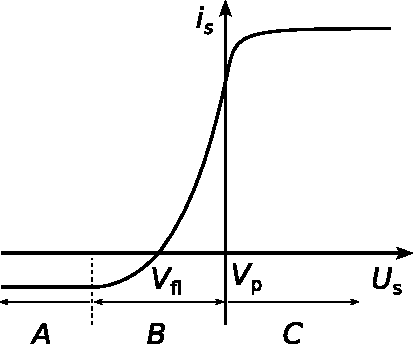
\includegraphics{vac-simple}
	\caption{Voltampérová charakteristika jednoduché sondy.
		Převzato z~\autocite{assignment-simpleprobe}.}
	\label{fig:vac-simple}
\end{figure}

\subsubsection{Oblast saturovaného proudu \parta}
Pokud je sonda výrazně záporně nabitá vzhledem k potenciálu plazmatu,
uplatní se Debyeovo stínění a~v~okolí sondy vznikne vrstva kladného
prostorového náboje.
Jelikož v této vrstvě nejsou elektrony, nemůže zde probíhat rekombinace,
ionizace, ani excitace nárazem elektronu a kolem sondy pozorujeme temný prostor.
Proud dopadající na sondu je převážně iontový
a~jeho velikost se řídí Child-Langmuirovým zákonem.

\subsubsection{Přechodová oblast \partb}
Při zvýšení napětí na sondě získají některé elektrony dostatečnou energii na to,
aby překonaly stěnovou vrstvu a dopadly na povrch sondy.
Iontový proud stále převládá.
Absolutní hodnota proudu s~rostoucím napětím na sondě klesá.
Bod, pro nějž je roven nule (tedy tam, kde se proudové příspěvky vyrovnají)
se nazývá plovoucí potenciál $\flpot$.
Další zvyšování napětí na sondě $\potprobe$ má za následek růst celkového proudu.
Zde již převládá proud elektronový $\ielec$, jehož průběh v~této oblasti lze
za předpokladu Maxwell-Boltzmannova rozdělení popsat vztahem:
\begin{equation}
	\label{eq:partb}
	\ielec = \probesurf \elemcharge \denselec
		\sqrt{\frac{\boltzmann \tempelec}{2 \pi \masselec}}
		e^{\frac{-\elemcharge\uprobe}{\boltzmann \tempelec}},
\end{equation}
kde $\probesurf$ je plocha sondy, $\denselec$ koncentrace elektronů,
$\boltzmann$ Boltzmanova konstanta, $\tempelec$ elektronová teplota,
$\elemcharge$~elementární náboj a~$\masselec$ hmotnost elektronu.
Nastává změna polarizace sondy.
Ze~vztahu \eqref{eq:partb} plyne,
že závislost $\ln(\ielec)=f(\uprobe)$ by měla být lineární.
Směrnice přímky potom určuje teplotu elektronů $\tempelec$
a~konstantní člen koncentraci elektronů $\denselec$.

\subsubsection{Oblast saturovaného elektronového proudu \partc}
Je-li překročeno nulové napětí $\uprobe$ na sondě
(tedy je-li sonda nabita vzhledem k potenciálu plazmatu $\plpot$ kladně),
začíná sonda přitahovat elektrony a odpuzovat kladné ionty.

V~případě válcové sondy proud v~této oblasti parabolicky roste.

\section{Jednoduchá sonda}
\label{sec:simple}

\subsection{Metoda}
\label{sec:method-simple}
Schéma měřicí aparatury je na obrázku č.~\ref{fig:diagram-simple}.
Elektrody ve válcové výbojové trubici jsou připojeny k~laditelnému zdroji
stejnostměrného napětí a výbojový proud $\idisch$ je snímán ampérmetrem.
Válcová sonda o~poloměru $r=\SI{0.1}{\milli\metre}$
a délce $l=\SI{8}{\milli\metre}$ je umístěna poblíž anody.
Sondový obvod je napájen stejnosměrným zdrojem s~automatizovaým laděním.
Potenciál sondy $\potprobe$ a~sondový proud $\iprobe$ jsou měřeny
voltmetrem a~přesným ampérmetrem připojeným k~počítači.

\begin{figure}[hbp]
	\centering
	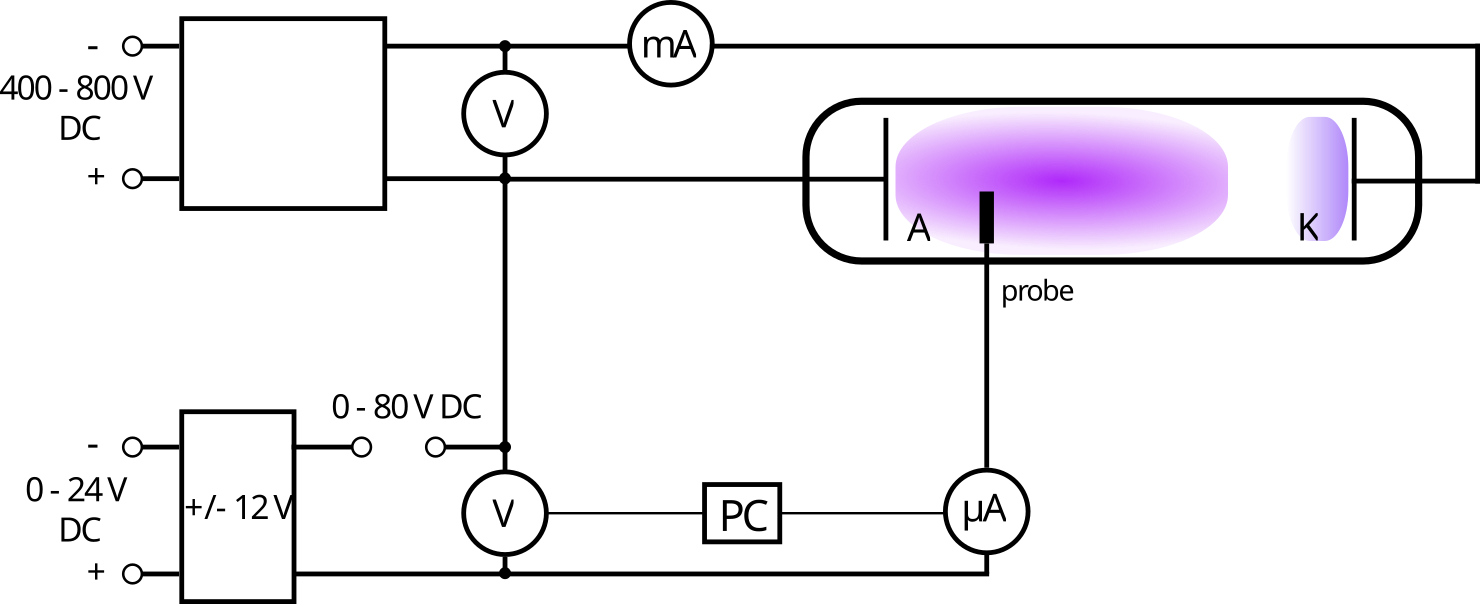
\includegraphics{diagram-simple.png}
	\caption{Uspořádání experimentu pro jednoduchou sondu.
		Převzato z~\autocite{assignment-simpleprobe}.}
	\label{fig:diagram-simple}
\end{figure}

Pro každou sadu podmínek byl nejprve přibližně určen plovoucí potenciál sondy
$\flpot$ jako bod, v~němž je proud sondou $\iprobe$ nulový.
Voltampérová charakteristika byla následně naměřena v~rozsahu~\SI{20}{\volt}
kolem plovoucího potenciálu.
Potenciál sondy byl automaticky lineárně zvyšován z~nejnižší hodnoty
na~nejvyšší a~zpět, čímž byly získány dvě datové sady.
Z~datových sad byly vyřazeny ty, u~nichž došlo k~nevysvětlenému kolísání
sondového proudu.
Kde zůstaly obě sady pro stejné podmínky, byly získány dvě voltampérové
charakteristiky, které byly zprůměrovány,

Hodnoty $\potprobe$ a~$\iprobe$ byly asynchronně zaznamenávány počítačem
spolu s~časovými značkami, které umožnily přiřazení odpovídajících hodnot
napětí a~proudu.
Vzhledem k~zaokrouhlení časových údajů na celé sekundy lze očekávat
nepřesnost přiřazení dat v~řádu desetin sekundy.

\subsubsection{Elektronový proud}
Levá část získané voltampérové charakteristiky byla proložena lineární funkcí
a~extrapolována pro celou oblast, kde nabývala záporných hodnot
(což nastalo pro všechny hodnoty potenciálu $\potprobe$).
Tato funkce byla považována za iontovou část sondového proudu $\iion$.
Elektronový proud byl získán odečtením iontového proudu od celkového:
\begin{equation}
	\label{eq:ielec}
	\ielec = \iprobe - \iion.
\end{equation}

\subsubsection{Plazmový potenciál}
Potenciál neporušeného plazmatu $\plpot$ byl určen dvěma metodami.
První z~nich bylo stanovení tohoto potenciálu jako průsečíku přímek
proložených střední a~koncovou částí elektronového proudu v~logaritmickém
měřítku.

Druhá metoda vychází z~poznatku, že v~okolí plazmového potenciálu $\plpot$
bude mít voltampérová charakteristika inflexní bod:
Elektronový proud byl kvůli potlačení šumu vyhlazen polynomem osmého stupně
a plazmový potenciál byl stanoven jako nulový bod druhé derivace $\didu$
proloženého polynomu.

\subsubsection{Elektronová teplota}
Ze směrnice přímky proložené střední částí charakteristiky byla určena
elektronová teplota $\tempelec$ podle vztahu:
\begin{equation}
	\label{eq:tempeleca}
	\tempeleca = \frac{\elemcharge}{\boltzmann \slopeb},
\end{equation}
kde $\slopeb$ je směrnice proložené přímky.
%
Pro porovnání byla elektronová teplota určena také z~plovoucího potenciálu
$\flpot$ jako:
\begin{equation}
	\label{eq:tempelecp}
	\tempelecp = \frac{2\elemcharge}{\boltzmann}
		\ln\left(\frac{4\pi\masselec}{\massion}\right)
		|\flpot - \plpot|,
\end{equation}
kde $\massion$ je hmotnost iontu pracovního plynu.

\subsection{Výsledky}
\label{results-simple}
Naměřené voltampérové charakteristiky jsou na obrázcích
č.~\ref{fig:simple1-vac-1}--\ref{fig:simple1-vac-6}.

\newcommand\figvac[3]{
	\begin{figure}[htp]
		\centering
		\input{plots/simple1-vac-#1}
		\input{plots/simple1-vac-log-#1}
		\caption{Voltampérová charakteristika sondy
			při výbojovém proudu $\idisch = \SI{#2}{\milli\ampere}$
			a tlaku $\pres = \SI{#3}{\pascal}$.}
		\label{fig:simple1-vac-#1}
	\end{figure}
}

\figvac{1}{50}{50}
\figvac{2}{40}{50}
\figvac{3}{30}{50}

\figvac{7}{50}{100}
\figvac{4}{50}{20}
\figvac{5}{50}{10}
\figvac{6}{50}{5}

\clearpage
\section{Jednoduchá sonda s~oscilujícím napětím}
\label{sec:eedf}

\subsection{Metoda}
\label{sec:method-eedf}
Modifikace zapojení popsaného v~části \ref{sec:method-simple}
umožňuje stanovit derivaci $\didu$ jinou cestou.
K~napětí na sondě je přidána malá střídavá složka $\ueedf\,\sin{\omega t}$,
která způsobí nárůst sondového proudu přibližně o~hodnotu:
\begin{equation}
	\label{eq:eedf-idiff}
	\Delta\iprobe = \frac{\ueedf^2}{4}\didu.
\end{equation}
Schéma tohoto zapojení je na obrázku č.~\ref{fig:diagram-eedf}.

\begin{figure}[hbp]
	\centering
	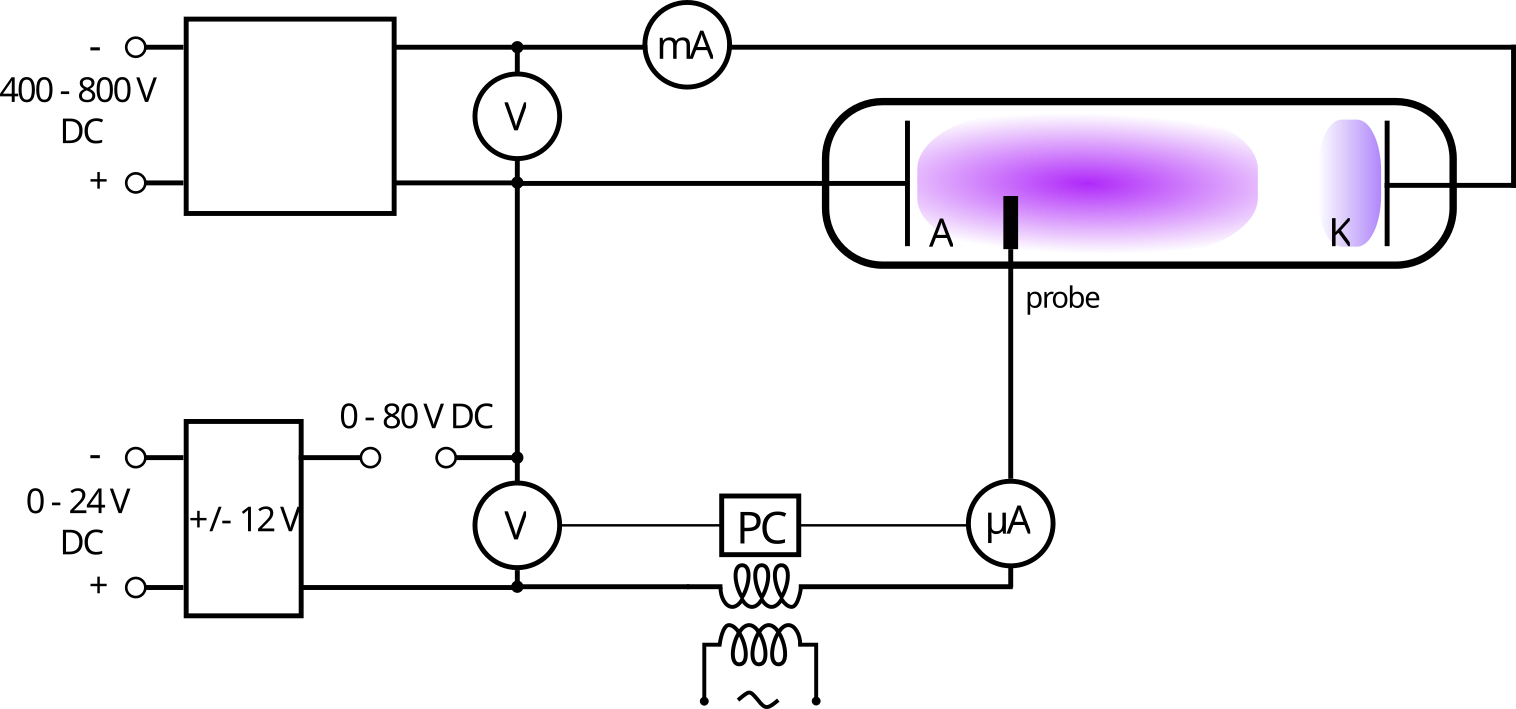
\includegraphics{diagram-eedf.png}
	\caption{Uspořádání experimentu pro jednoduchou sondu se střídavým napětím.
		Převzato z~\autocite{assignment-simpleprobe}.}
	\label{fig:diagram-eedf}
\end{figure}

\subsubsection{Rozdělovací funkce elektronů}
Rozdělovací funkce elektronů podle energie $\eedf$ byla určena ze vztahu:
\begin{equation}
	\label{eq:eedf}
	\eedf = \frac{1}{A} \sqrt{\frac{8\,\masselec}{\elemcharge^3}\,|\uprobe|}
		\,\frac{\mathrm d^2 \ielec}{\mathrm d\uprobe^2},
\end{equation}
kde $A$ je plocha sondy, $\masselec$ je hmotnost elektronu
a $\elemcharge$ elementární náboj.
Derivace voltampérové charakteristiky byla spočtena z~naměřených dat
po vyhlazení polynomem osmého stupně.

\subsection{Výsledky}
\label{sec:results-eedf}

\begin{figure}[p]
	\centering
	\input{plots/simple2-vac-1}
	\input{plots/simple2-vac-log-1}
	\input{plots/simple2-vac-2}
	\input{plots/simple2-vac-log-2}
	\input{plots/simple2-vac-3}
	\input{plots/simple2-vac-log-3}
	\caption{Voltampérové charakteristiky jednoduché sondy
		v~zapojení s~oscilujícím napětím
		pro měření rozdělovací funkce elektronů.
		$\idisch$ je výbojový proud a~$\pres$ je tlak.}
	\label{fig:simple2-vac}
\end{figure}

\begin{figure}
	\centering
	\input{plots/simple2-eedf-1}
	\input{plots/simple2-eedf-2}
	\input{plots/simple2-eedf-3}
	\caption{Rozdělovací funkce elektronů $\eedf$ podle energie.}
	\label{fig:eedf}
\end{figure}

\printbibliography
\end{document}
